% !TeX root = ../hw4.tex
\section{Reproducing the Book's Fractal Plants}

\subsection{Statement}
Use bracketed OL-systems to reproduce each of the plant-like fractals in Figure 7.24 of the book.

Experiment with the production rules and produce at least ten derivatives.

\subsection{Method}
The methods here are no different than Section \ref{sec:l-system-method}.

\subsection{Implementation}
The implementation is identical to Section \ref{sec:l-sys-implementation}.

\subsection{Results}\label{sec:p2-results}

\begin{figure}[H]
    \centering
    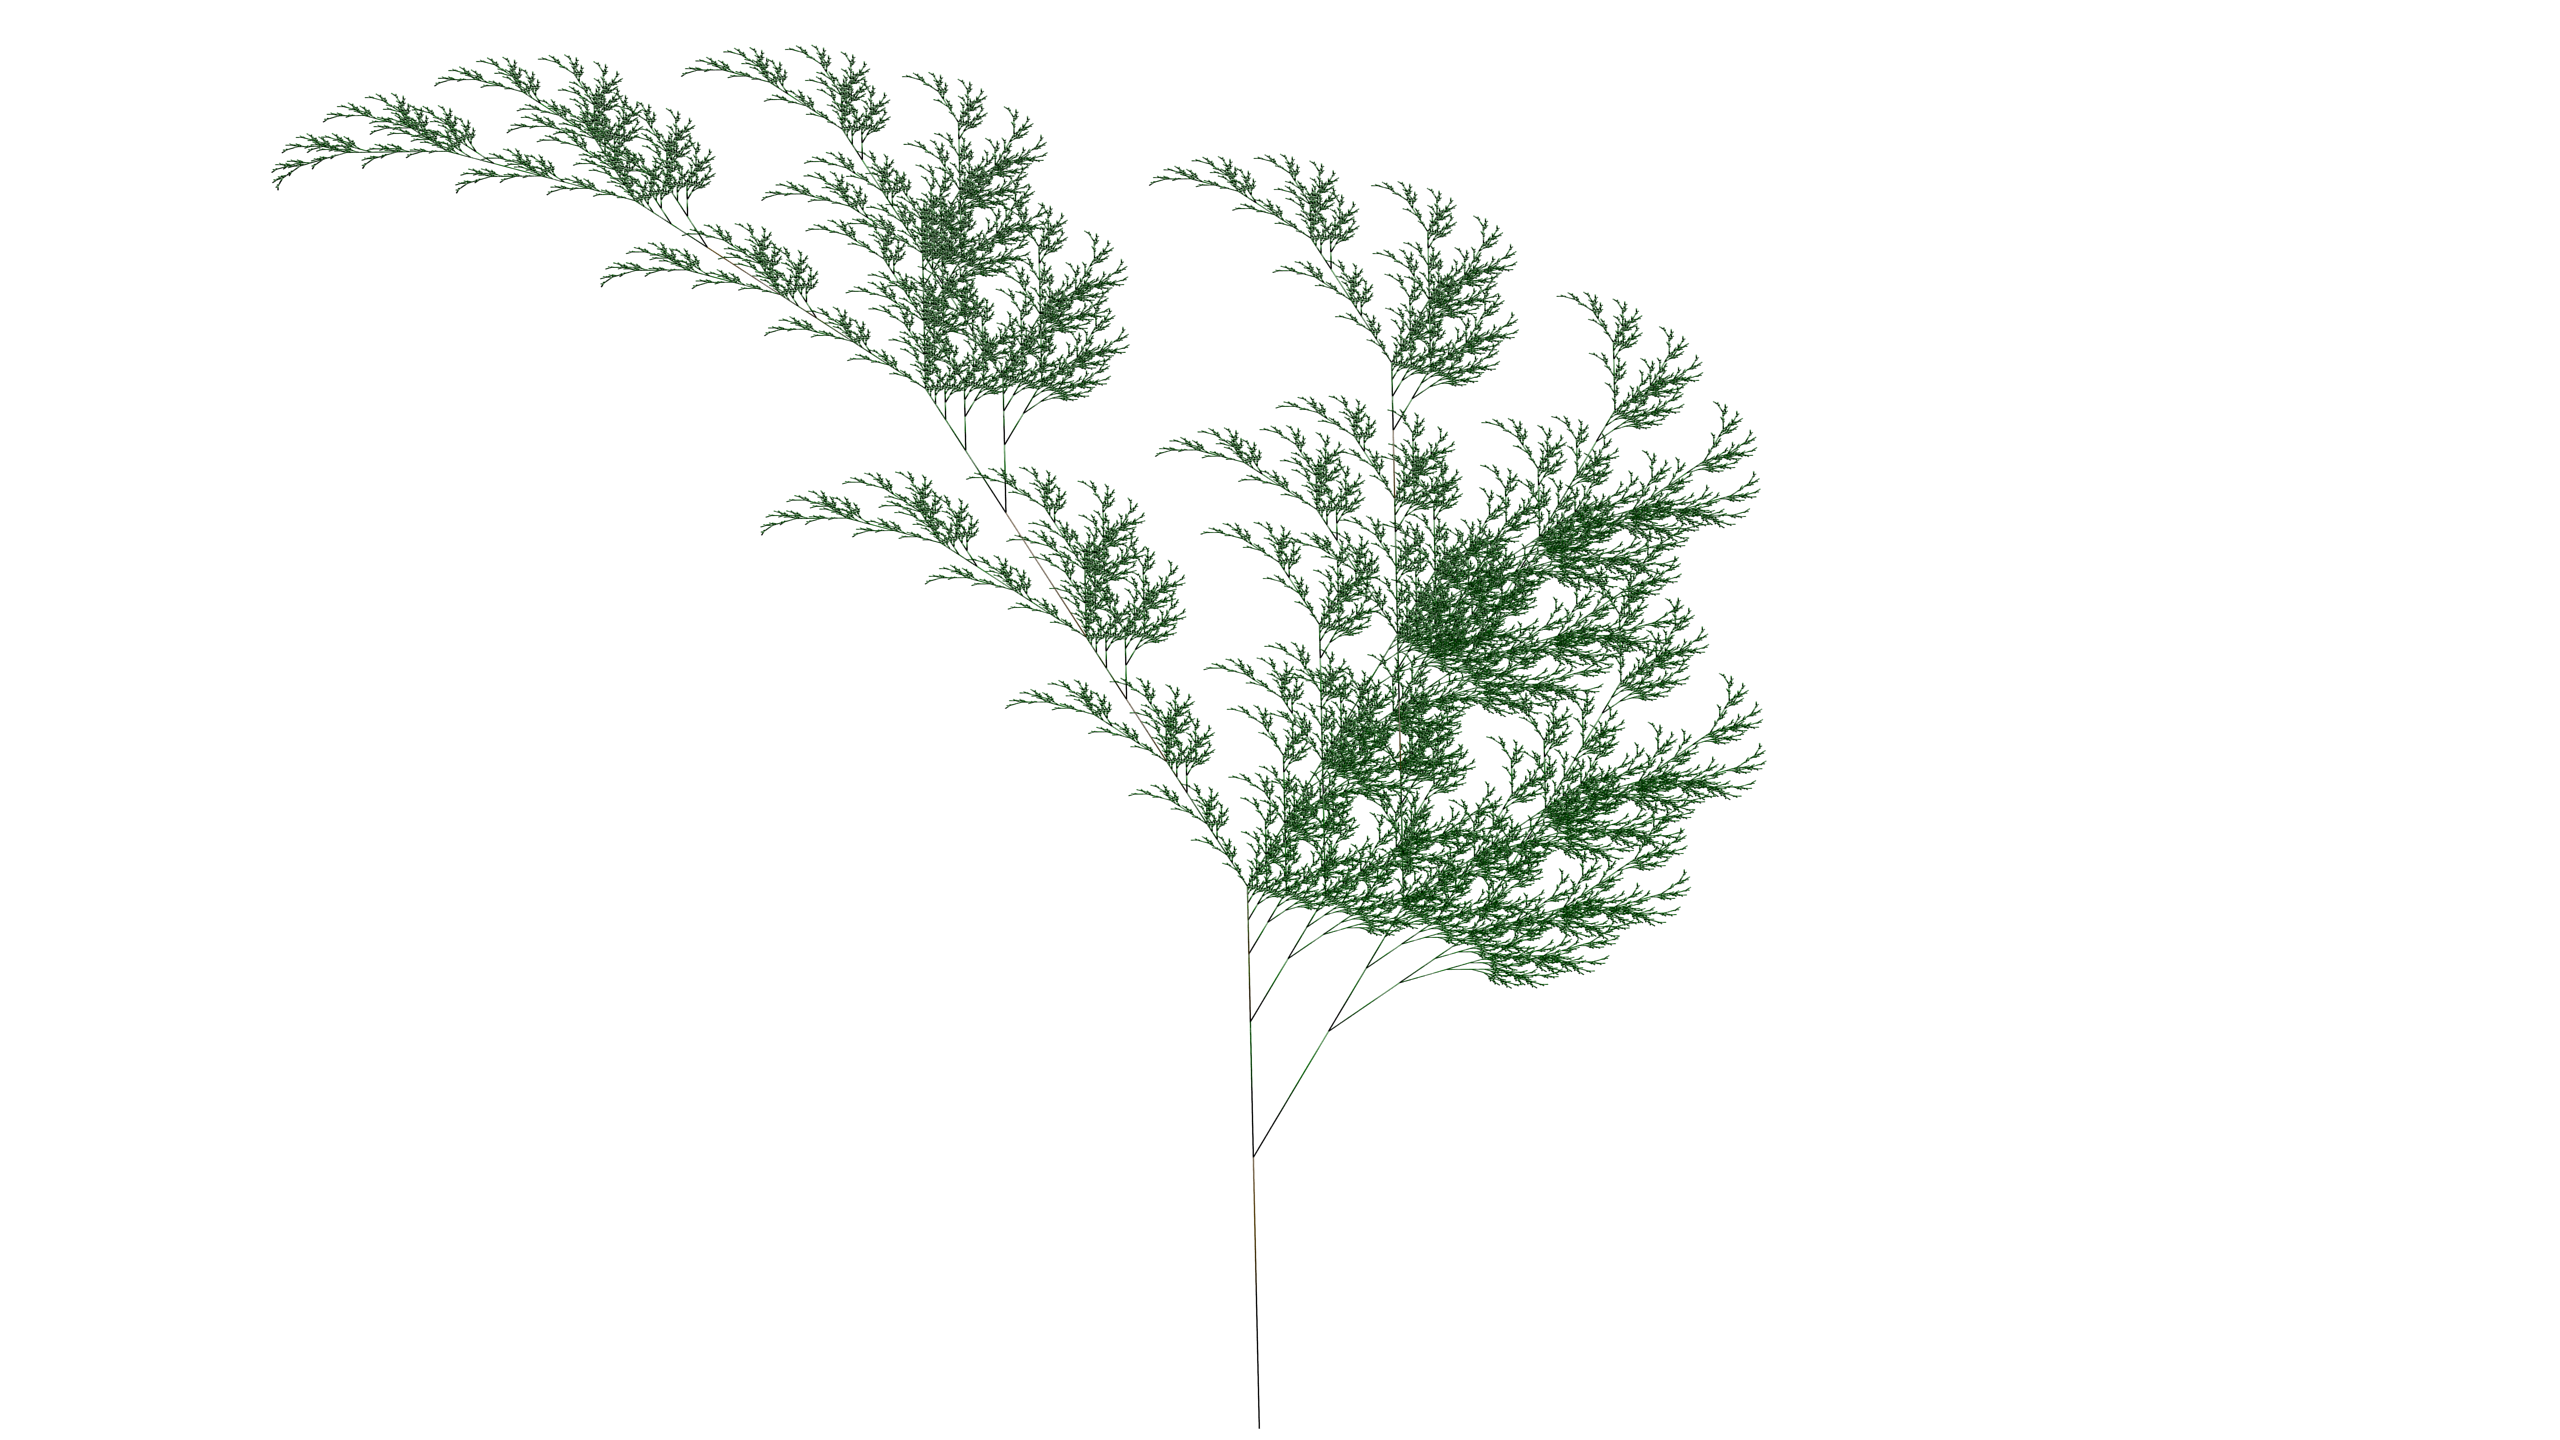
\includegraphics[width=0.90\textwidth]{figures/L-systems/a.png}
    \caption{Problem 2a}\label{fig:prob2a}
\end{figure}

\begin{figure}[H]
    \centering
    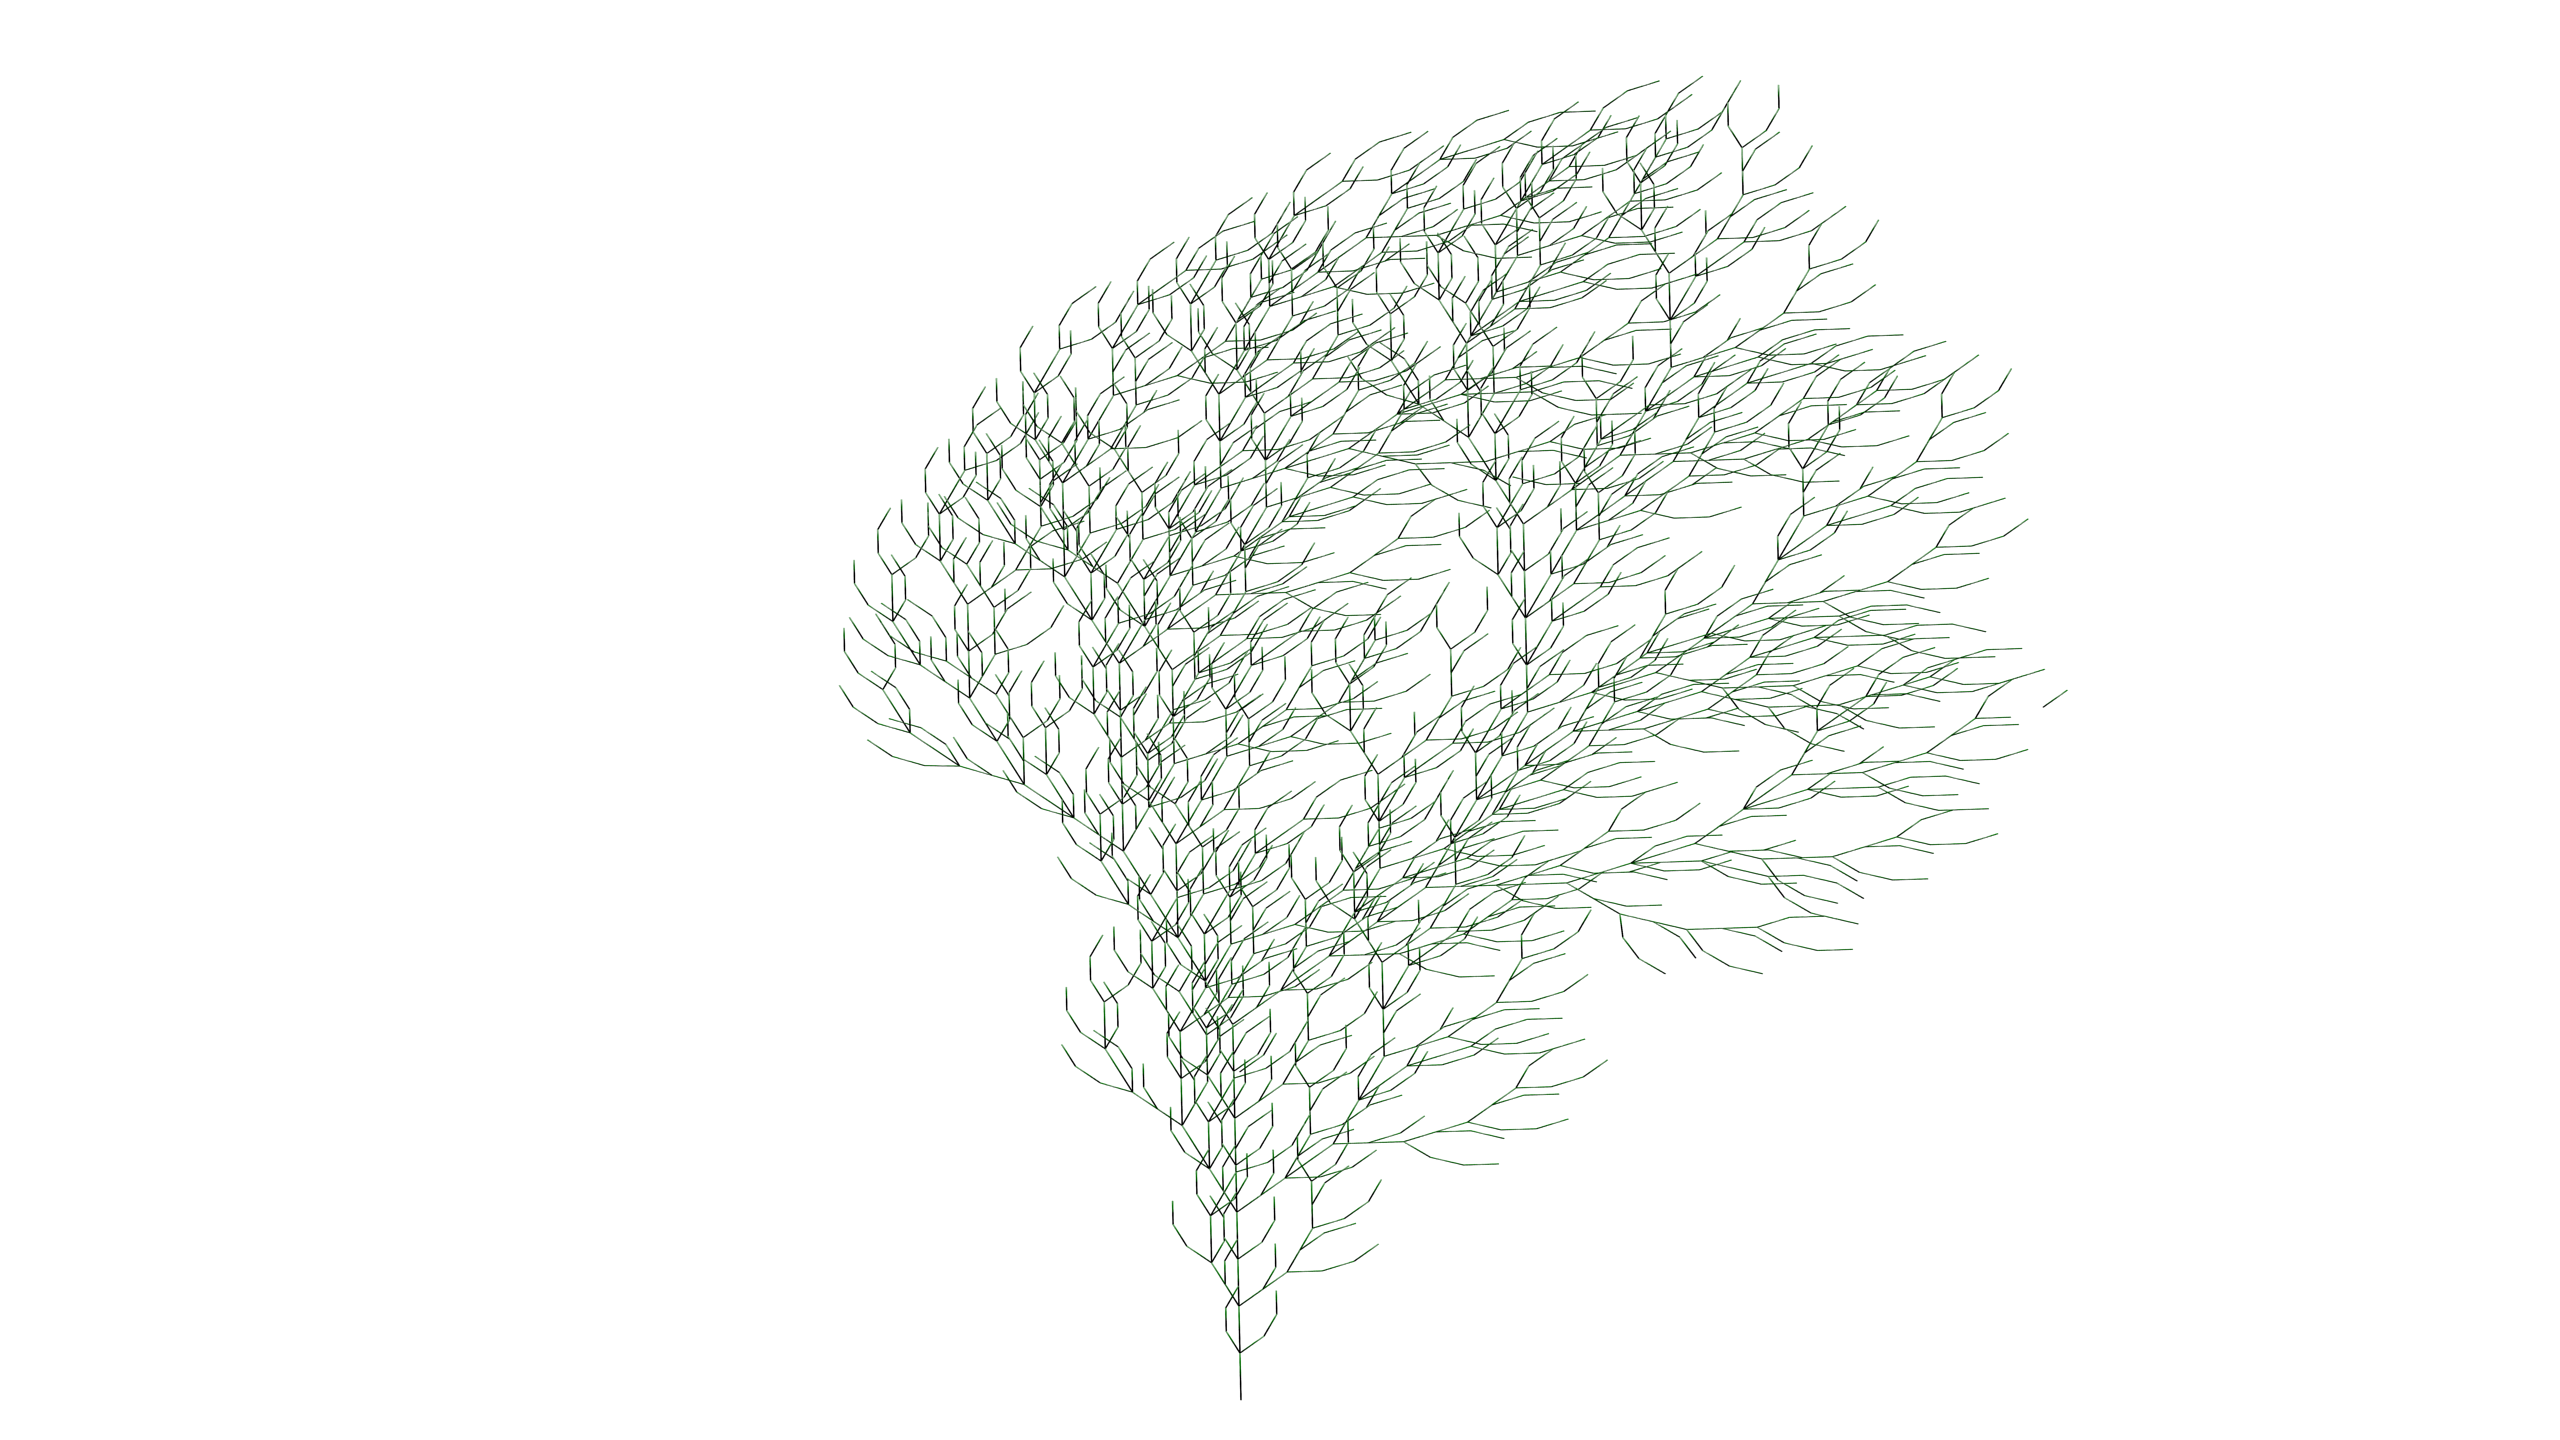
\includegraphics[width=0.90\textwidth]{figures/L-systems/b.png}
    \caption{Problem 2b}\label{fig:prob2b}
\end{figure}

\begin{figure}[H]
    \centering
    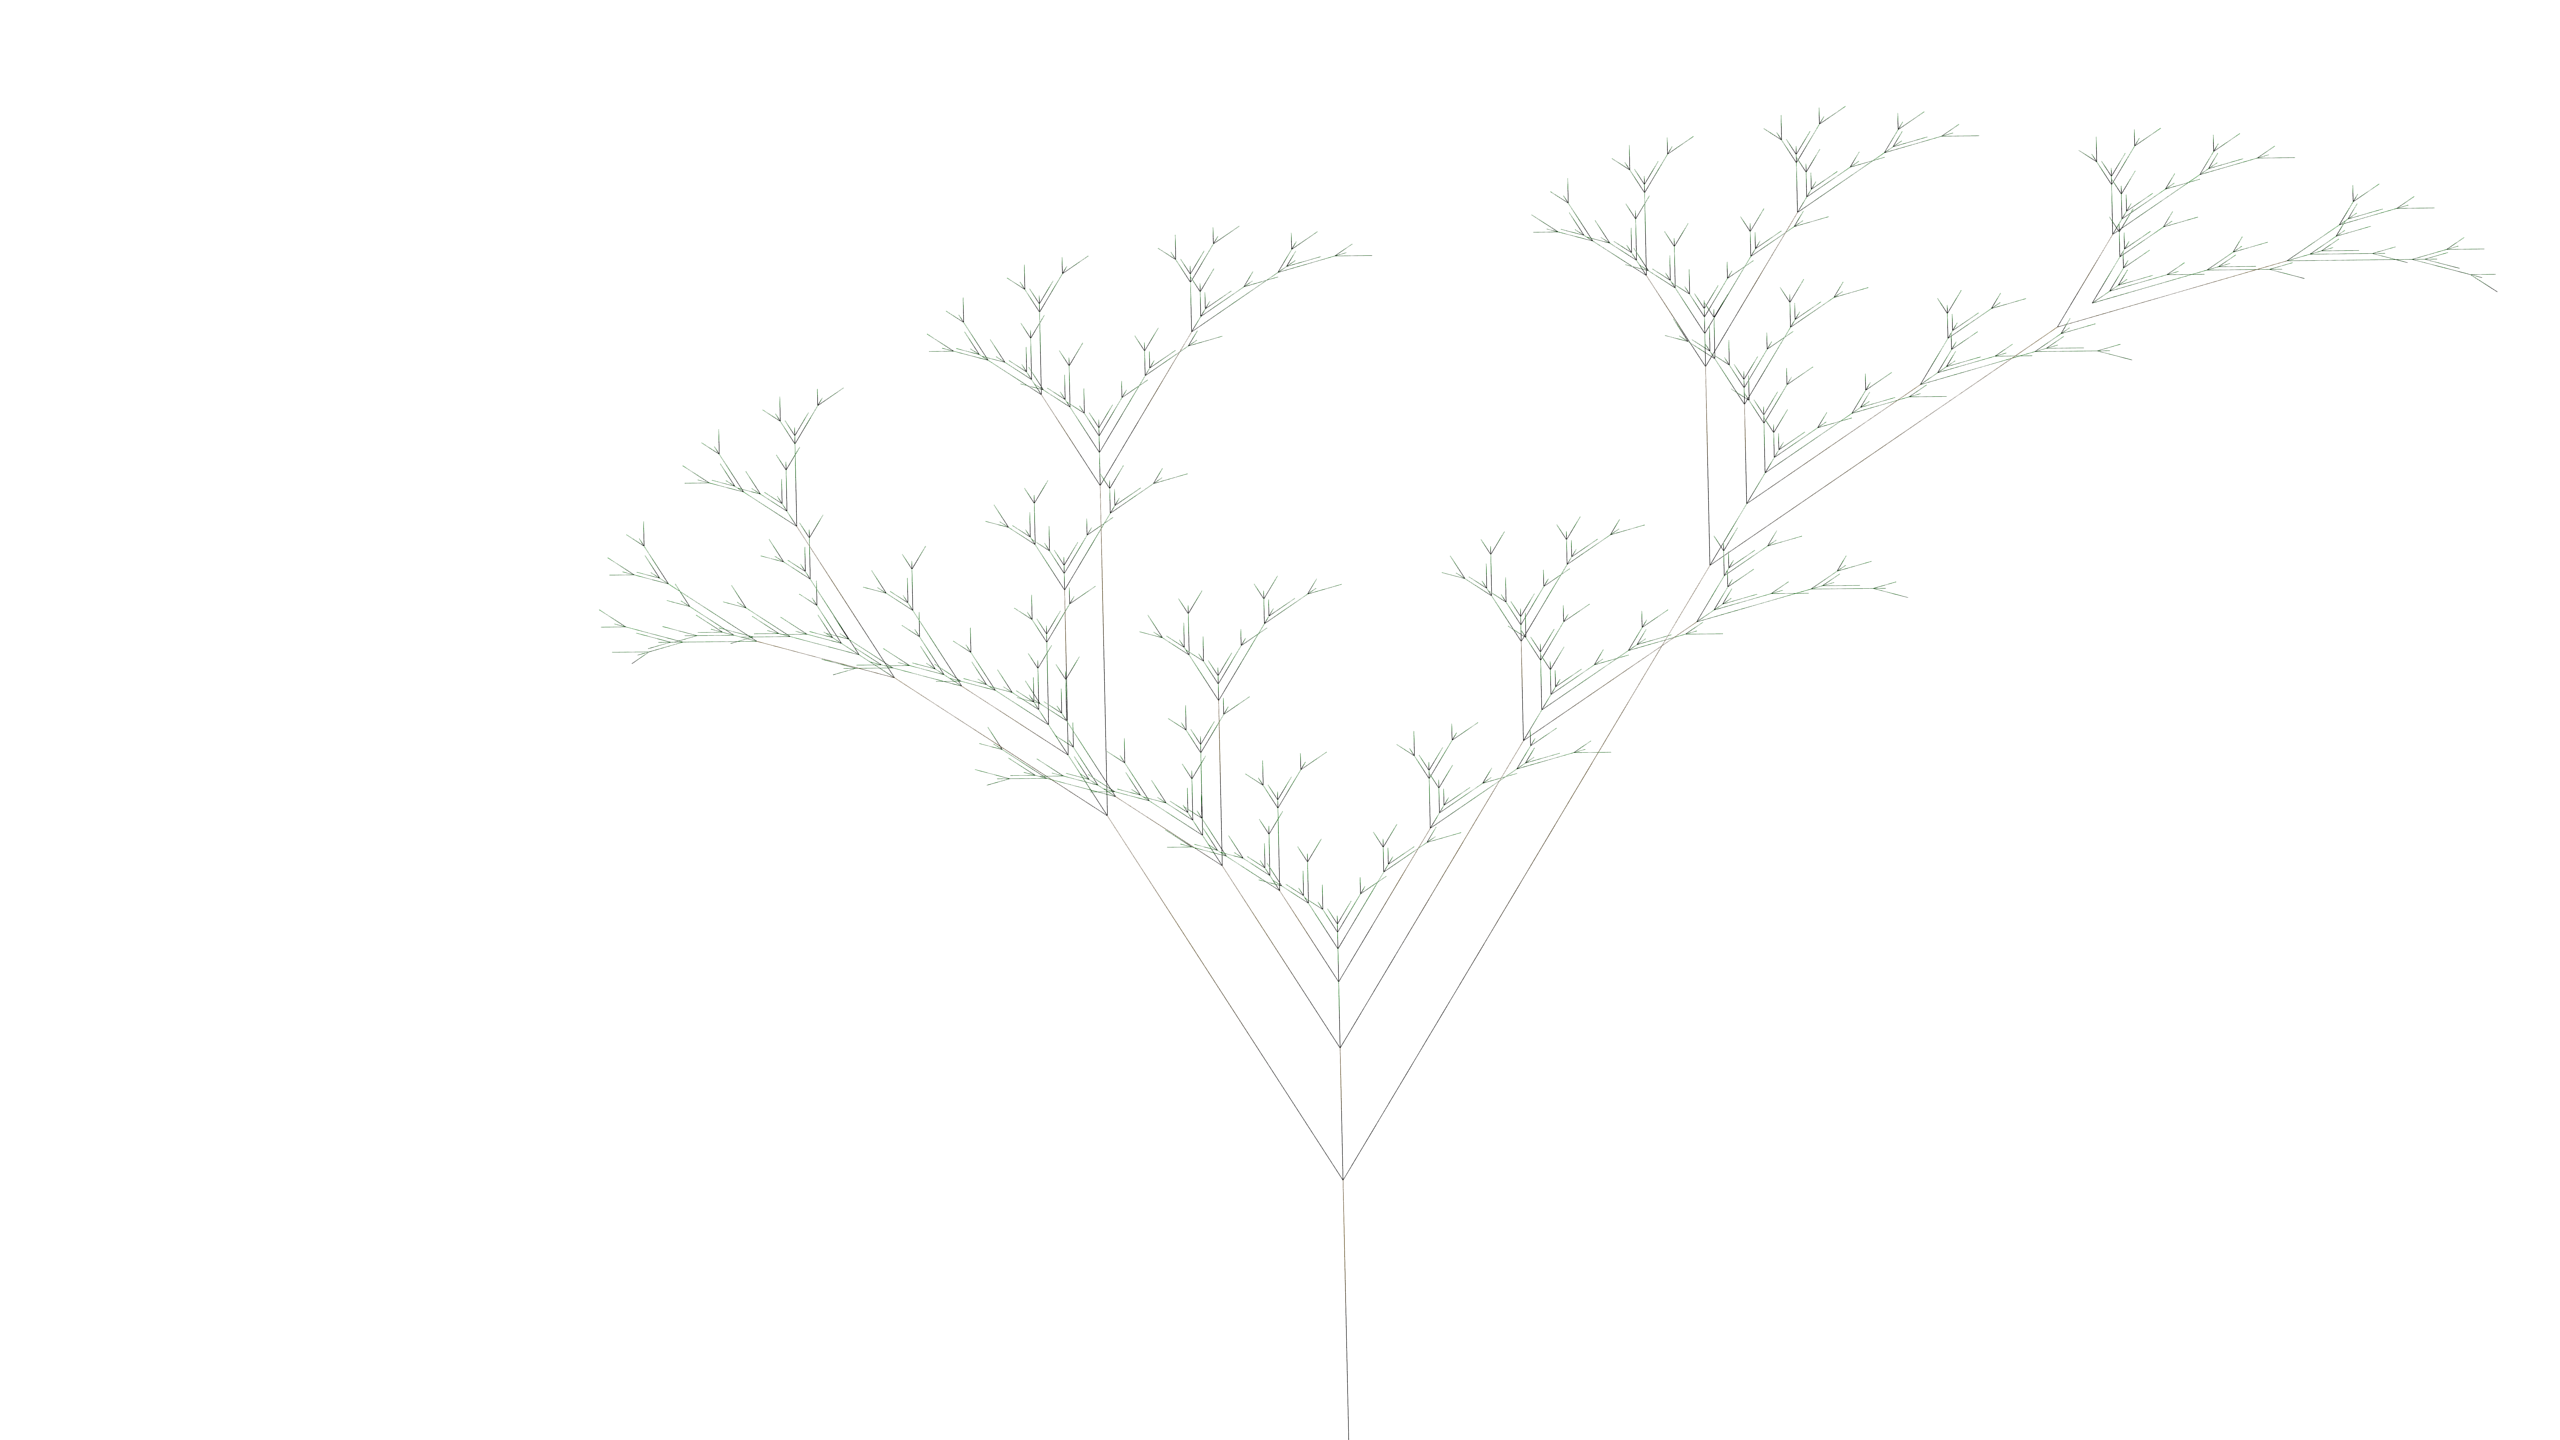
\includegraphics[width=0.90\textwidth]{figures/L-systems/c.png}
    \caption{Problem 2c}\label{fig:prob2c}
\end{figure}

\begin{figure}[H]
    \centering
    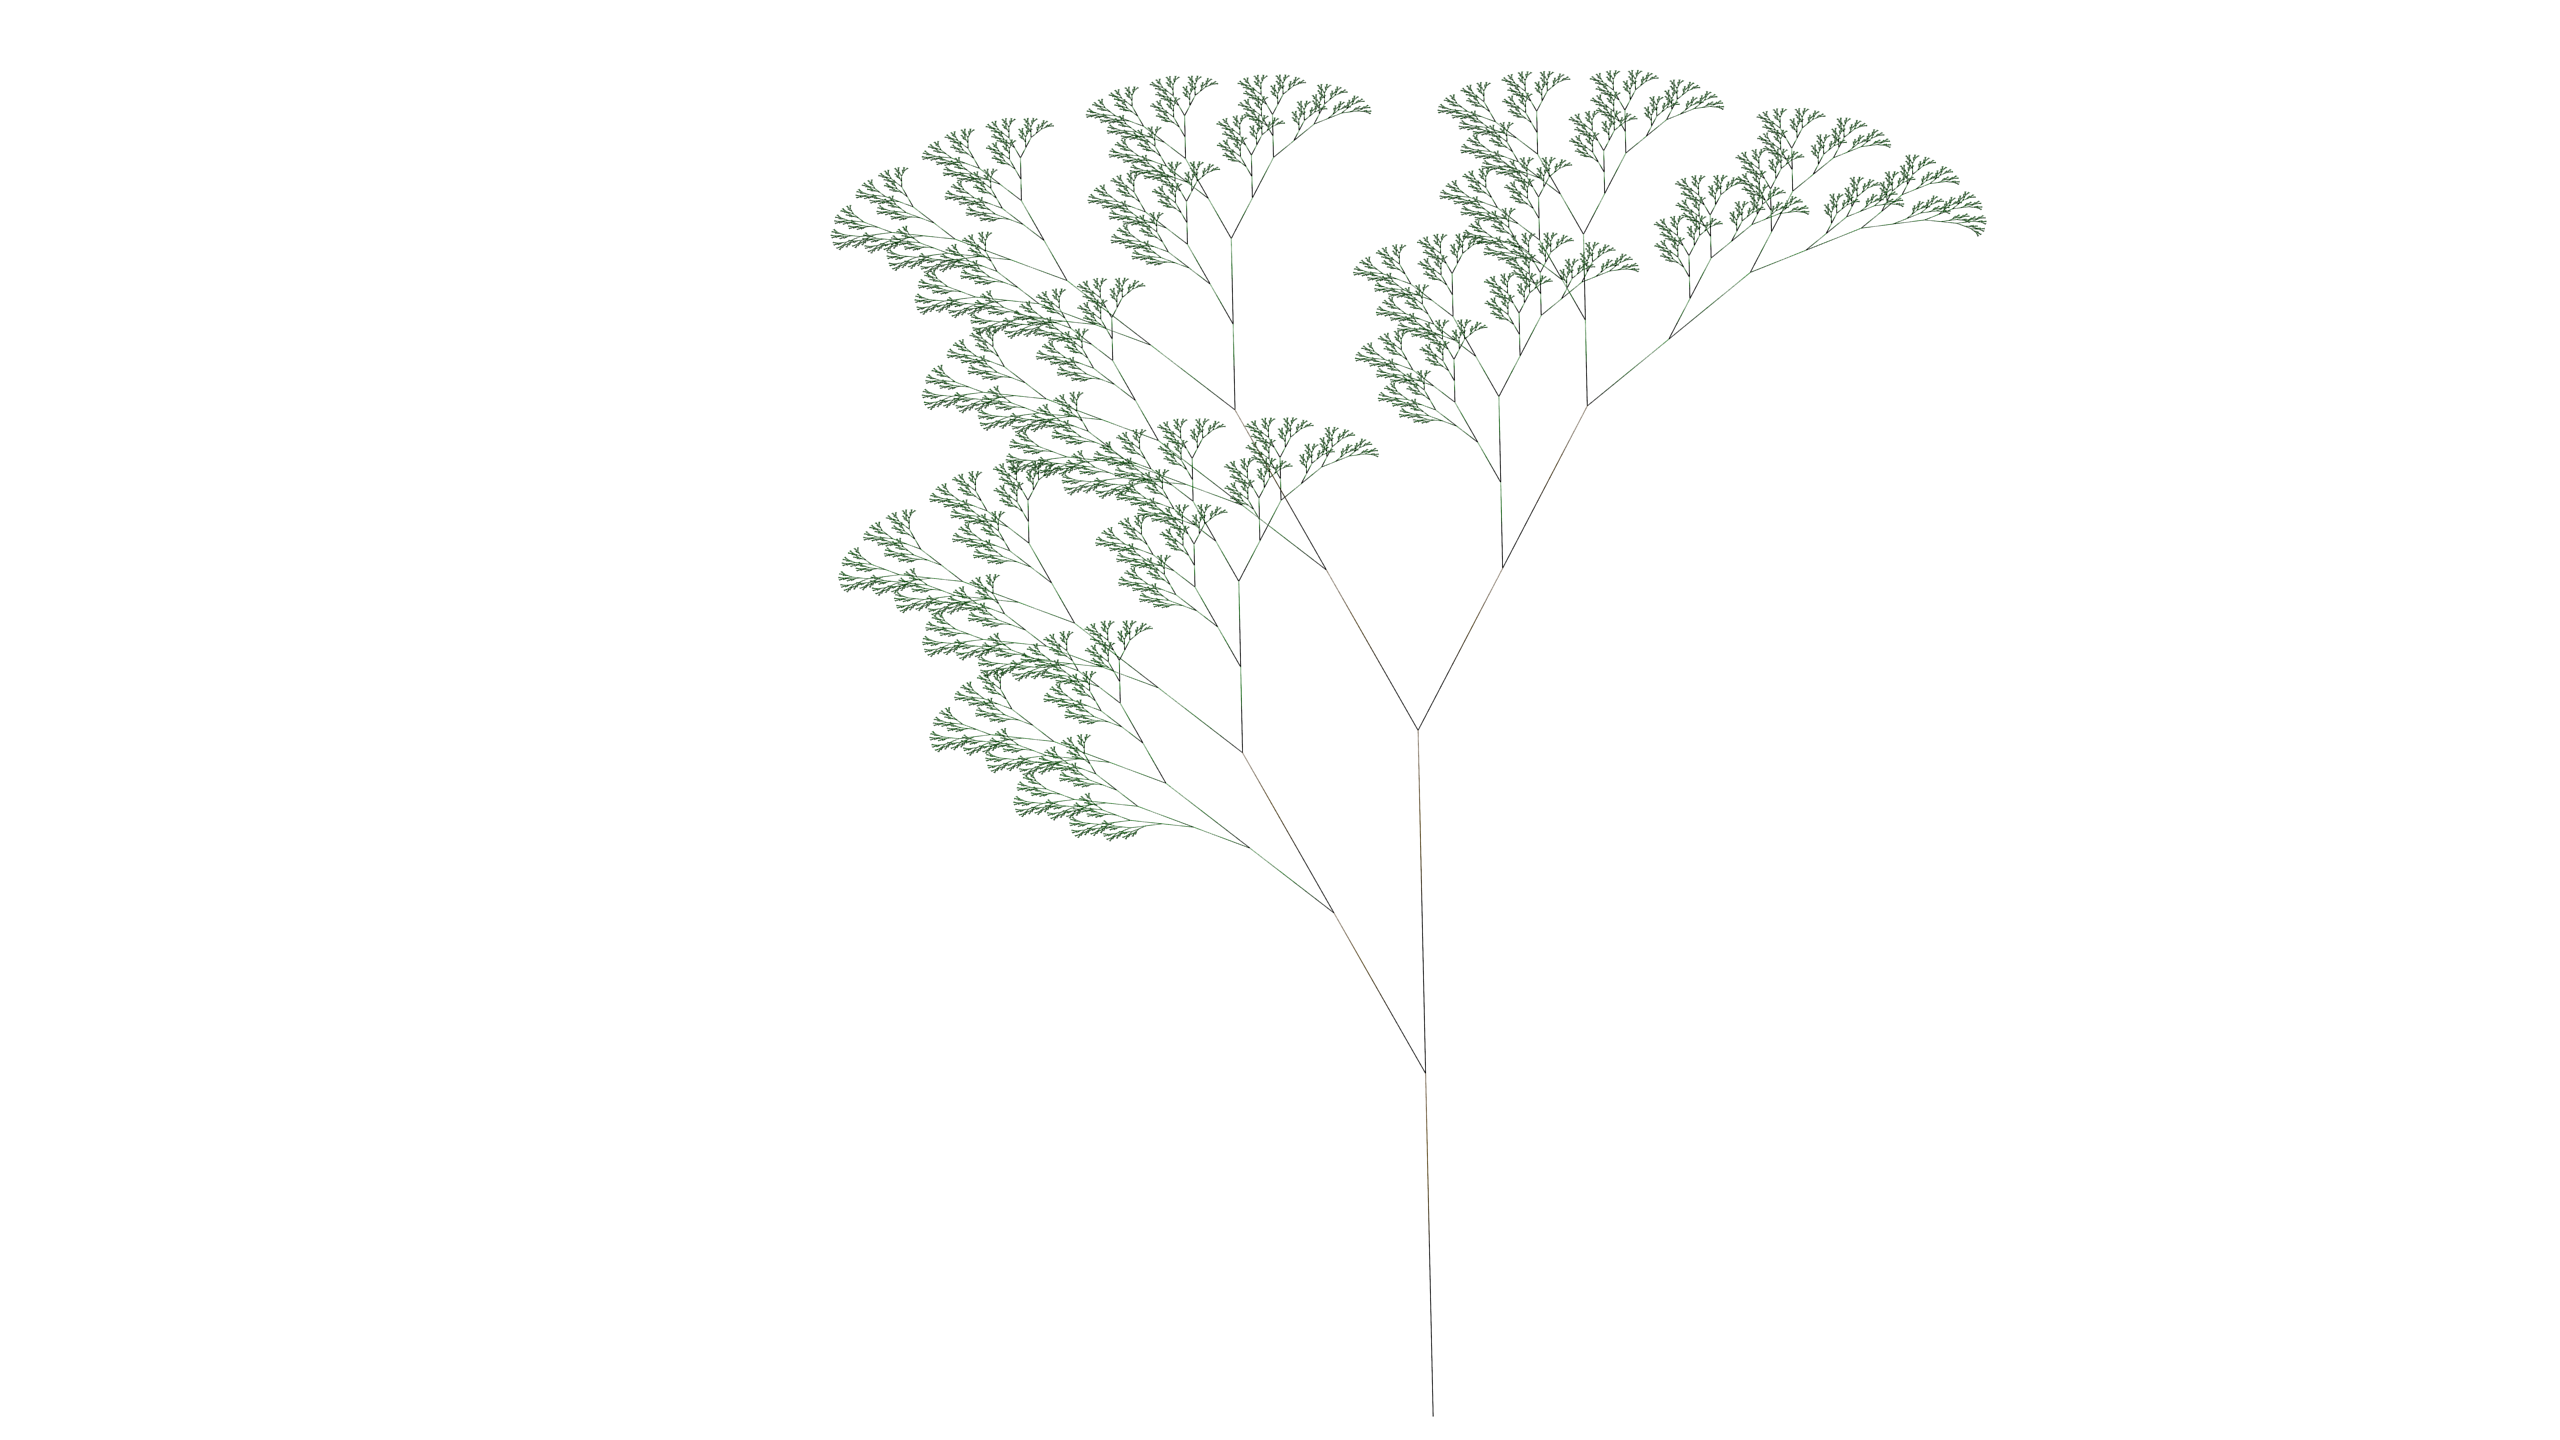
\includegraphics[width=0.90\textwidth]{figures/L-systems/d.png}
    \caption{Problem 2d}\label{fig:prob2d}
\end{figure}

\begin{figure}[H]
    \centering
    \noindent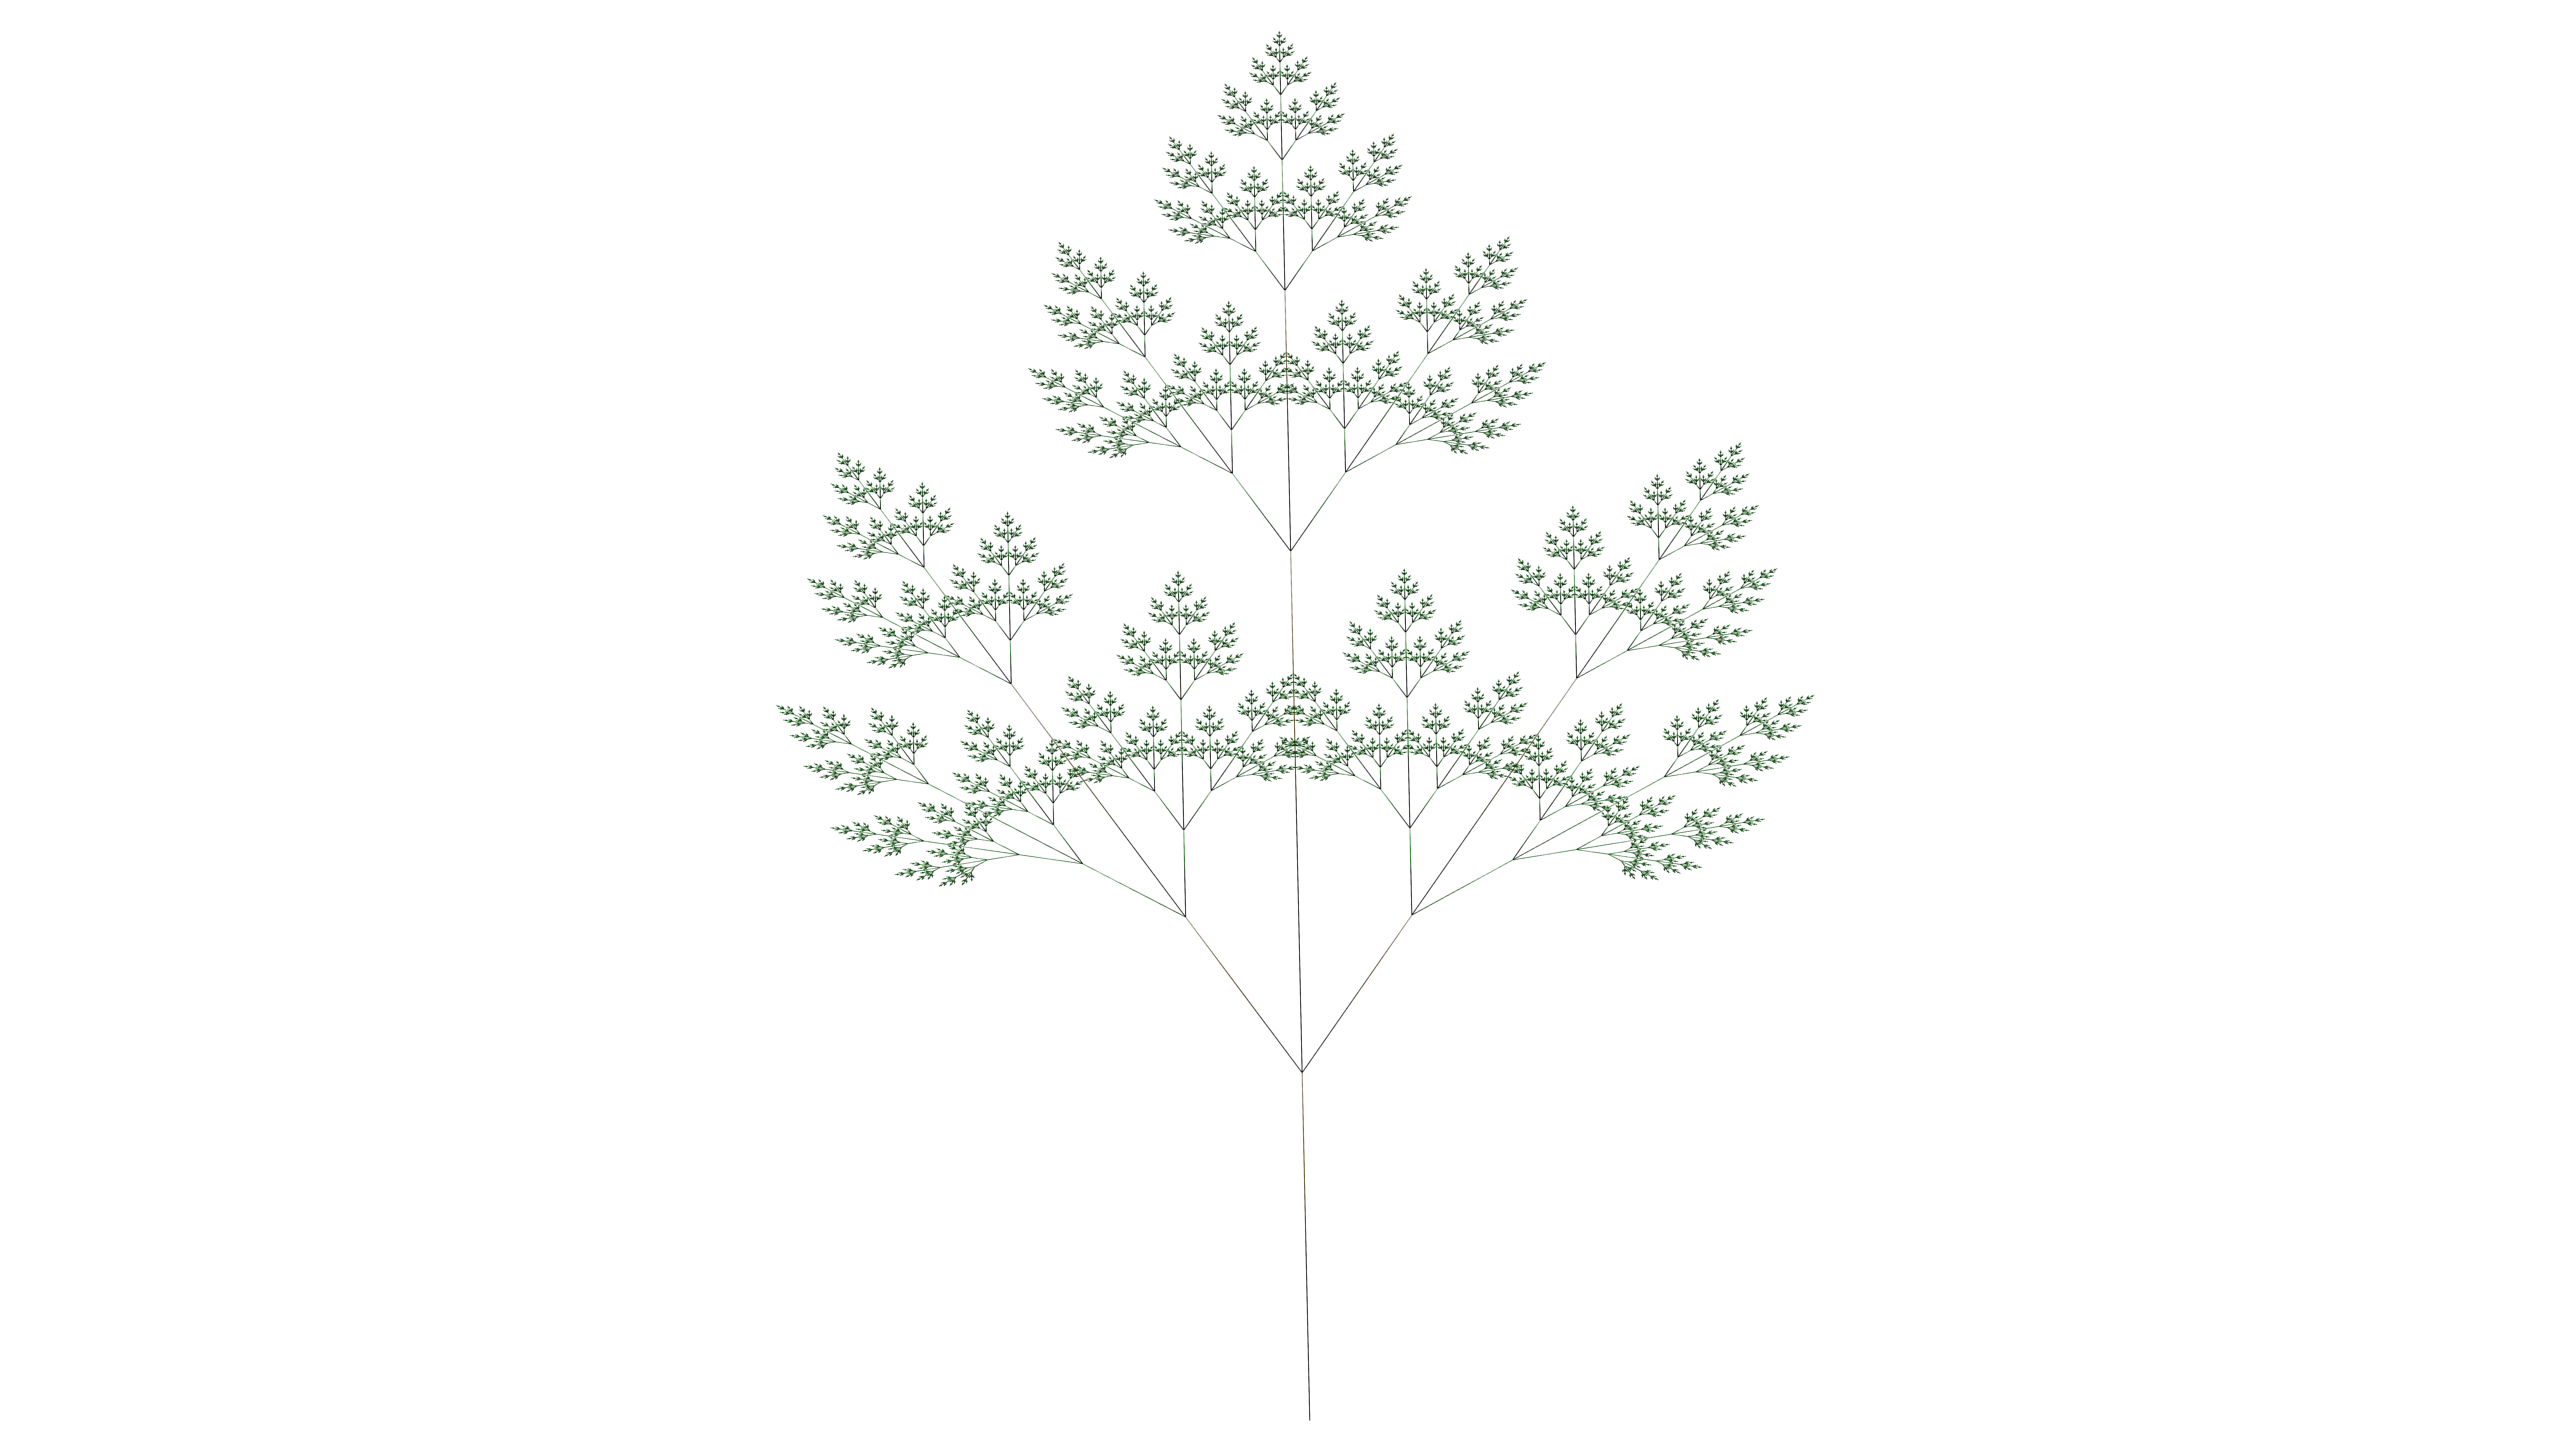
\includegraphics[width=0.90\textwidth]{figures/L-systems/e.png}
    \caption{Problem 2e}\label{fig:prob2e}
\end{figure}

\begin{figure}[H]
    \centering
    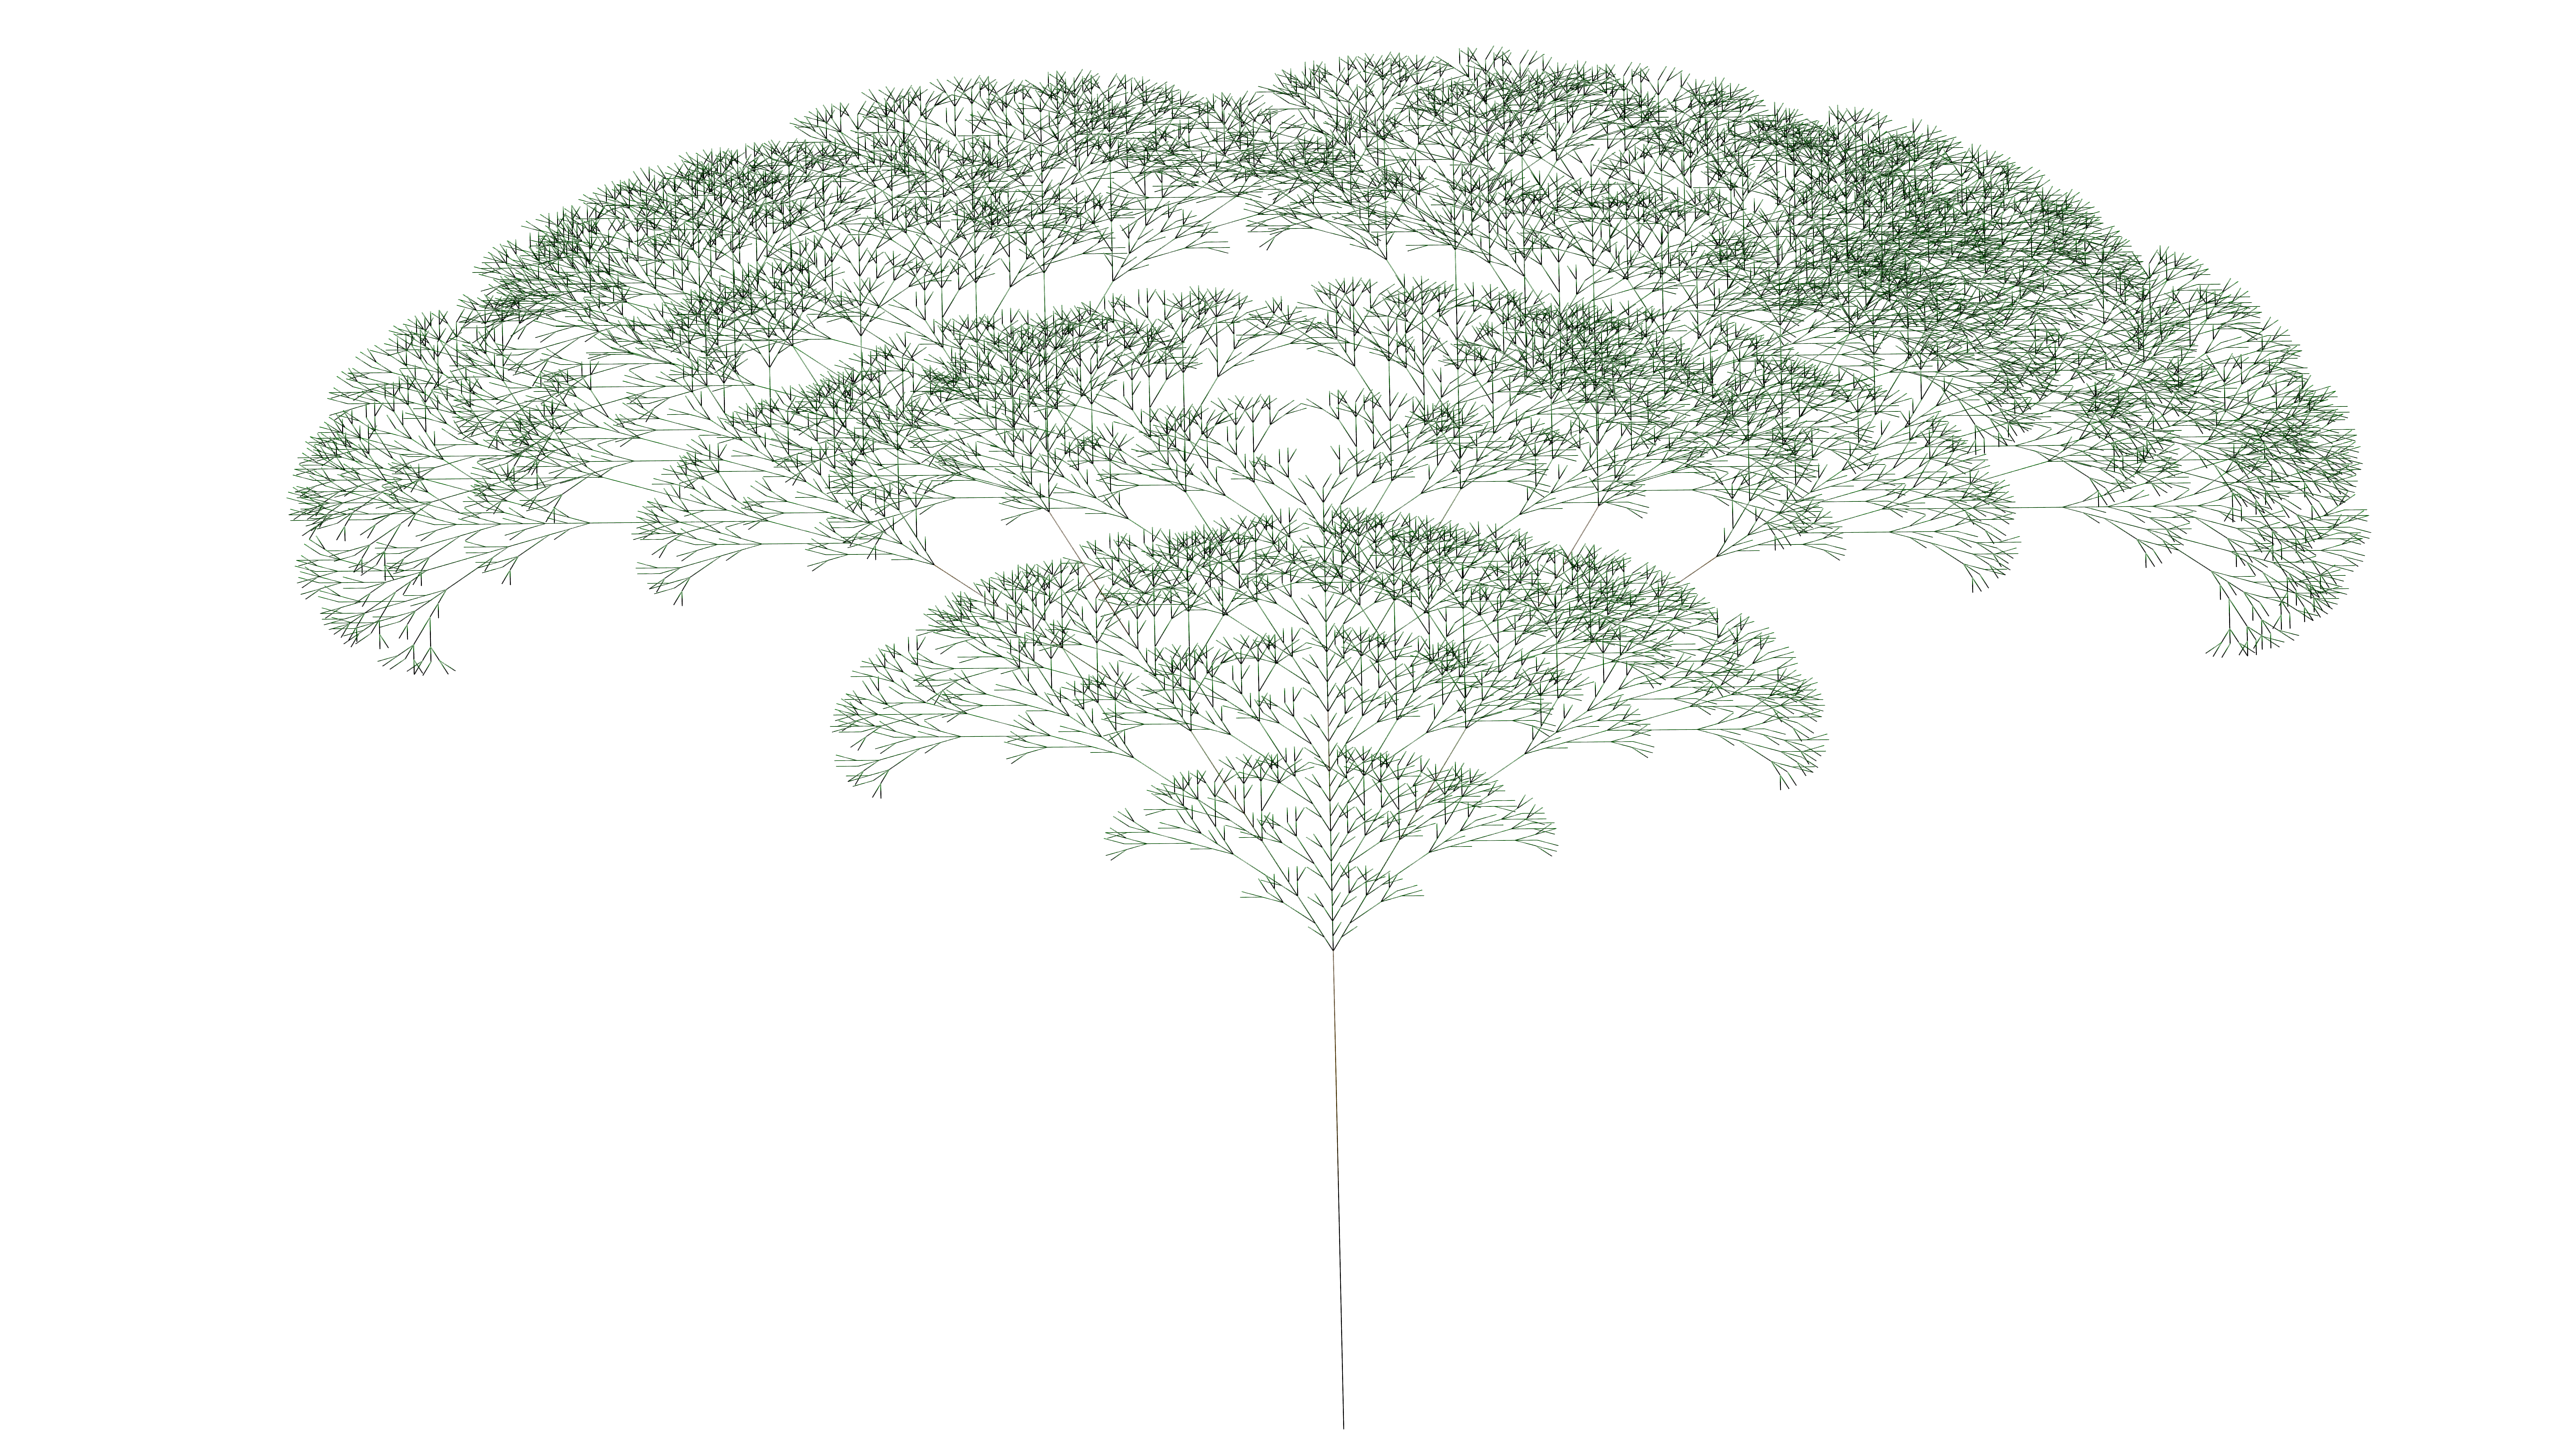
\includegraphics[width=0.90\textwidth]{figures/L-systems/f.png}
    \caption{Problem 2f}\label{fig:prob2f}
\end{figure}

\subsubsection{Expanding the Lindenmayer Systems to 3D}
We attempted to add an extra dimension to each of the items in Section
\ref{sec:p2-results}. We also experimented with classical systems such as
Sierpiński triangle, Cantor Set, Dragon, Koch, and variants of our own design.

% \todoinline[caption=3d results]{
%     Discuss how to create more interesting 3D fractals, including Koch curves, the dragon curve, and 3D trees/bushes.

%     Show the results from \texttt{data/a.json} with the book's parameters.
% }

\subsection{Conclusion}
Following the book examples were extremely simple to implement, we simply
created \texttt{JSON} files that matched the book description. To build the 3D
variants we experimented until they looked decent. The other variants were
through trial and error or online examples. It was fun to play with the
different rules and attempt to get structures that were uniform but didn't
entirely look uniform.
